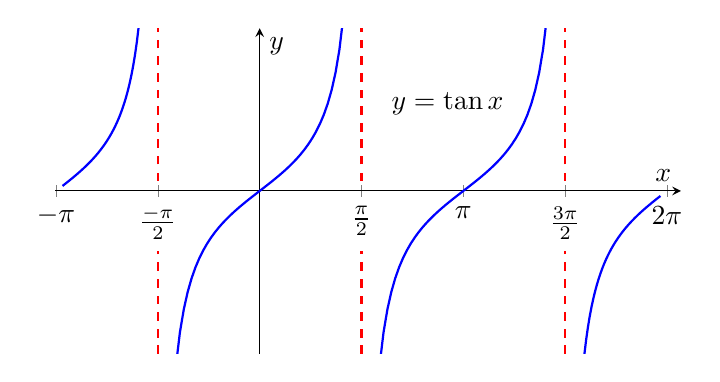
\begin{tikzpicture} 
\begin{axis}[
	width=3.75in,
	height=2.25in,
	axis lines = middle,
	xmin=-3.15, 
	xmax=6.5, 
	ymin=-3.25, 
	ymax=3.25, 
	xlabel=${x}$,
	ylabel=${y}$,
	xtick={-2*pi,-3*pi/2,-pi,-pi/2,pi/2,pi,3*pi/2,2*pi},
	ytick={-4,4},
	xticklabels = {${-2\pi}$,${\frac{-3\pi}{2}}$,${-\pi}$,${\frac{-\pi}{2}}$,${\frac{\pi}{2}}$,${\pi}$,${\frac{3\pi}{2}}$,${2\pi}$},
]
% defines the function
\addplot[  
	domain={pi/2+.1:3*pi/2-.1}, % the domain of the function
	blue, 
	thick,
	samples=50,
]
{tan(deg(x))};

\addplot[  
	domain={-pi+.1}:{-pi/2-.1}, % the domain of the function
	blue, 
	thick,
	samples=50,
]
{tan(deg(x))};

\addplot[  
	domain={3*pi/2+.1}:{2*pi-.1}, % the domain of the function
	blue, 
	thick,
	samples=50,
]
{tan(deg(x))};

\addplot[  
	domain={-pi/2+.1}:{pi/2-.1}, % the domain of the function
	blue, 
	thick,
	samples=50,
]
{tan(deg(x))};

\addplot[ % This is the parametric curve
	thick,
	dashed,
	variable=\t, % t is the parameter
	domain=-3.25:-1.2, % this is the domain of the parametric curve
    samples = 50,
    samples y=50,%prevents the starting and ending points from being joined by a line
	color=red,
]
({3*pi/2},{t});
\addplot[ % This is the parametric curve
	thick,
	dashed,
	variable=\t, % t is the parameter
	domain=-3.25:-1.2, % this is the domain of the parametric curve
    samples = 50,
    samples y=50,%prevents the starting and ending points from being joined by a line
	color=red,
]
({-pi/2},{t});


\addplot[ % This is the parametric curve
	thick,
	dashed,
	variable=\t, % t is the parameter
	domain=-3.25:-1.2, % this is the domain of the parametric curve
    samples = 50,
    samples y=50,%prevents the starting and ending points from being joined by a line
	color=red,
]
({pi/2},{t});

\addplot[ % This is the parametric curve
	thick,
	dashed,
	variable=\t, % t is the parameter
	domain=0.2:3.25, % this is the domain of the parametric curve
    samples = 50,
    samples y=50,%prevents the starting and ending points from being joined by a line
	color=red,
]
({3*pi/2},{t});
\addplot[ % This is the parametric curve
	thick,
	dashed,
	variable=\t, % t is the parameter
	domain=0.2:3.25, % this is the domain of the parametric curve
    samples = 50,
    samples y=50,%prevents the starting and ending points from being joined by a line
	color=red,
]
({-pi/2},{t});


\addplot[ % This is the parametric curve
	thick,
	dashed,
	variable=\t, % t is the parameter
	domain=0.2:3.25, % this is the domain of the parametric curve
    samples = 50,
    samples y=50,%prevents the starting and ending points from being joined by a line
	color=red,
]
({pi/2},{t});

\node at (axis cs:  2.9,1.75) {${\bm{y=\tan x}}$};


\end{axis}
\end{tikzpicture} 